%!TEX root = ../main.tex
\section{Pure random attachment}\label{section:pure-random-attachment}

\subsection{Degree distribution}
\subsubsection{Theory}
The pure random attachment model can be seen as a limiting case of the BA model. In this model, all existing vertices are chosen with equal probability, i.e. $\Pi = \Pi_{rnd} \propto 1$. This preserves growth but removes preferential attachment. 

Similar to the previous section, we start from the master equation in \autoref{eq:master}, and instead of $\Pi = k/ 2E(t)$ as in preferential attachment, we use $\Pi_{rnd} = 1 / N(t)$. Again, we consider the long-time ansatz $n(k, t) \rightarrow N(t) p_{\infty}(k)$. Substituting these terms into \autoref{eq:master}, we have

\begin{equation}
	p_{\infty}(k) = m p_{\infty}(k-1) - m p_{\infty}(k) + \delta_{k, m}. 
	\label{eq:ra-degree-distribution-p-infinity}
\end{equation}

Considering the case of $k > m$, we obtain the recurrence relation
\begin{equation}
	p_{\infty}(k) = \left ( \frac{m}{m+1} \right ) p_{\infty}(k-1)=...= \left ( \frac{m}{m+1} \right )^{k-m} p_{\infty}(m)
	\label{eq:ra-degree-recurrence-relation}
\end{equation}

Now we consider $k=m$. Substituting $k=m$ into \autoref{eq:ra-degree-distribution-p-infinity} and remembering that $p_{\infty}(k < m) = 0$, we get
\begin{equation}
	p_{\infty}(m) = -mp_{\infty} + 1, 
	\label{eq:ra-degree-k-equal-m}
\end{equation}
giving us 
\begin{equation}
	p_{\infty}(m) = \frac{1}{m+1}. 
	\label{eq:ra-degree-p-infinity-m}
\end{equation}

Combining this result with \autoref{eq:ra-degree-recurrence-relation}, we get the following formula for $p_{\infty}(k)$:
\begin{equation}
	p_{\infty}(k) = \frac{1}{m+1} \left ( \frac{m}{m+1}\right )^{k-m}.
	\label{eq:p-infinity-solution-ra}
\end{equation}

For normalization, we need to check that 
\begin{equation}
	\sum_{k=m}^{\infty}p_{\infty}(k) = \frac{1}{m+1} \sum_{k=m}^{\infty} \left ( \frac{m}{m+1}\right )^{k-m} = 1.
	\label{eq:ra-check-normalization}
\end{equation}
The terms in the summation form a converging geometric series, with the starting term being zero and common ratio being $m / (m+1)$. Hence we have 
\begin{equation}
	\sum_{k=m}^{\infty} \left ( \frac{m}{m+1} \right )^{k-m} = \frac{1}{1 - [m / (m+1)]}. 
	\label{eq:ra-geom-series}
\end{equation}

By substituting this back into the \autoref{eq:ra-check-normalization}, we can see that normalization is satisfied. 

As we can see from \autoref{eq:p-infinity-solution-ra}, the resulting degree distribution in this limit is geometric \citep{Pekoz2013}, indicating that growth alone is not sufficient to produce a scale free structure. 

\subsubsection{Numerical analysis}\label{subsection:ra-numerical-analysis}
Numerical simulations confirmed that growth alone is not sufficient to produce a scale free structure. \autoref{fig:ra-fixed-n-degree-dist} shows the raw degree distribution of numerical simulations for $N=10^6$ and different values of $m$. The fat tail was reduced by taking the average of multiple simulations. Already, we can see that it does not follow a power law. After log binning, it follows the theoretical geometric simulation very well for small $k$, as can be seen in \autoref{fig:ra-fixed-n-logbin}.

\begin{figure}
    \centering
    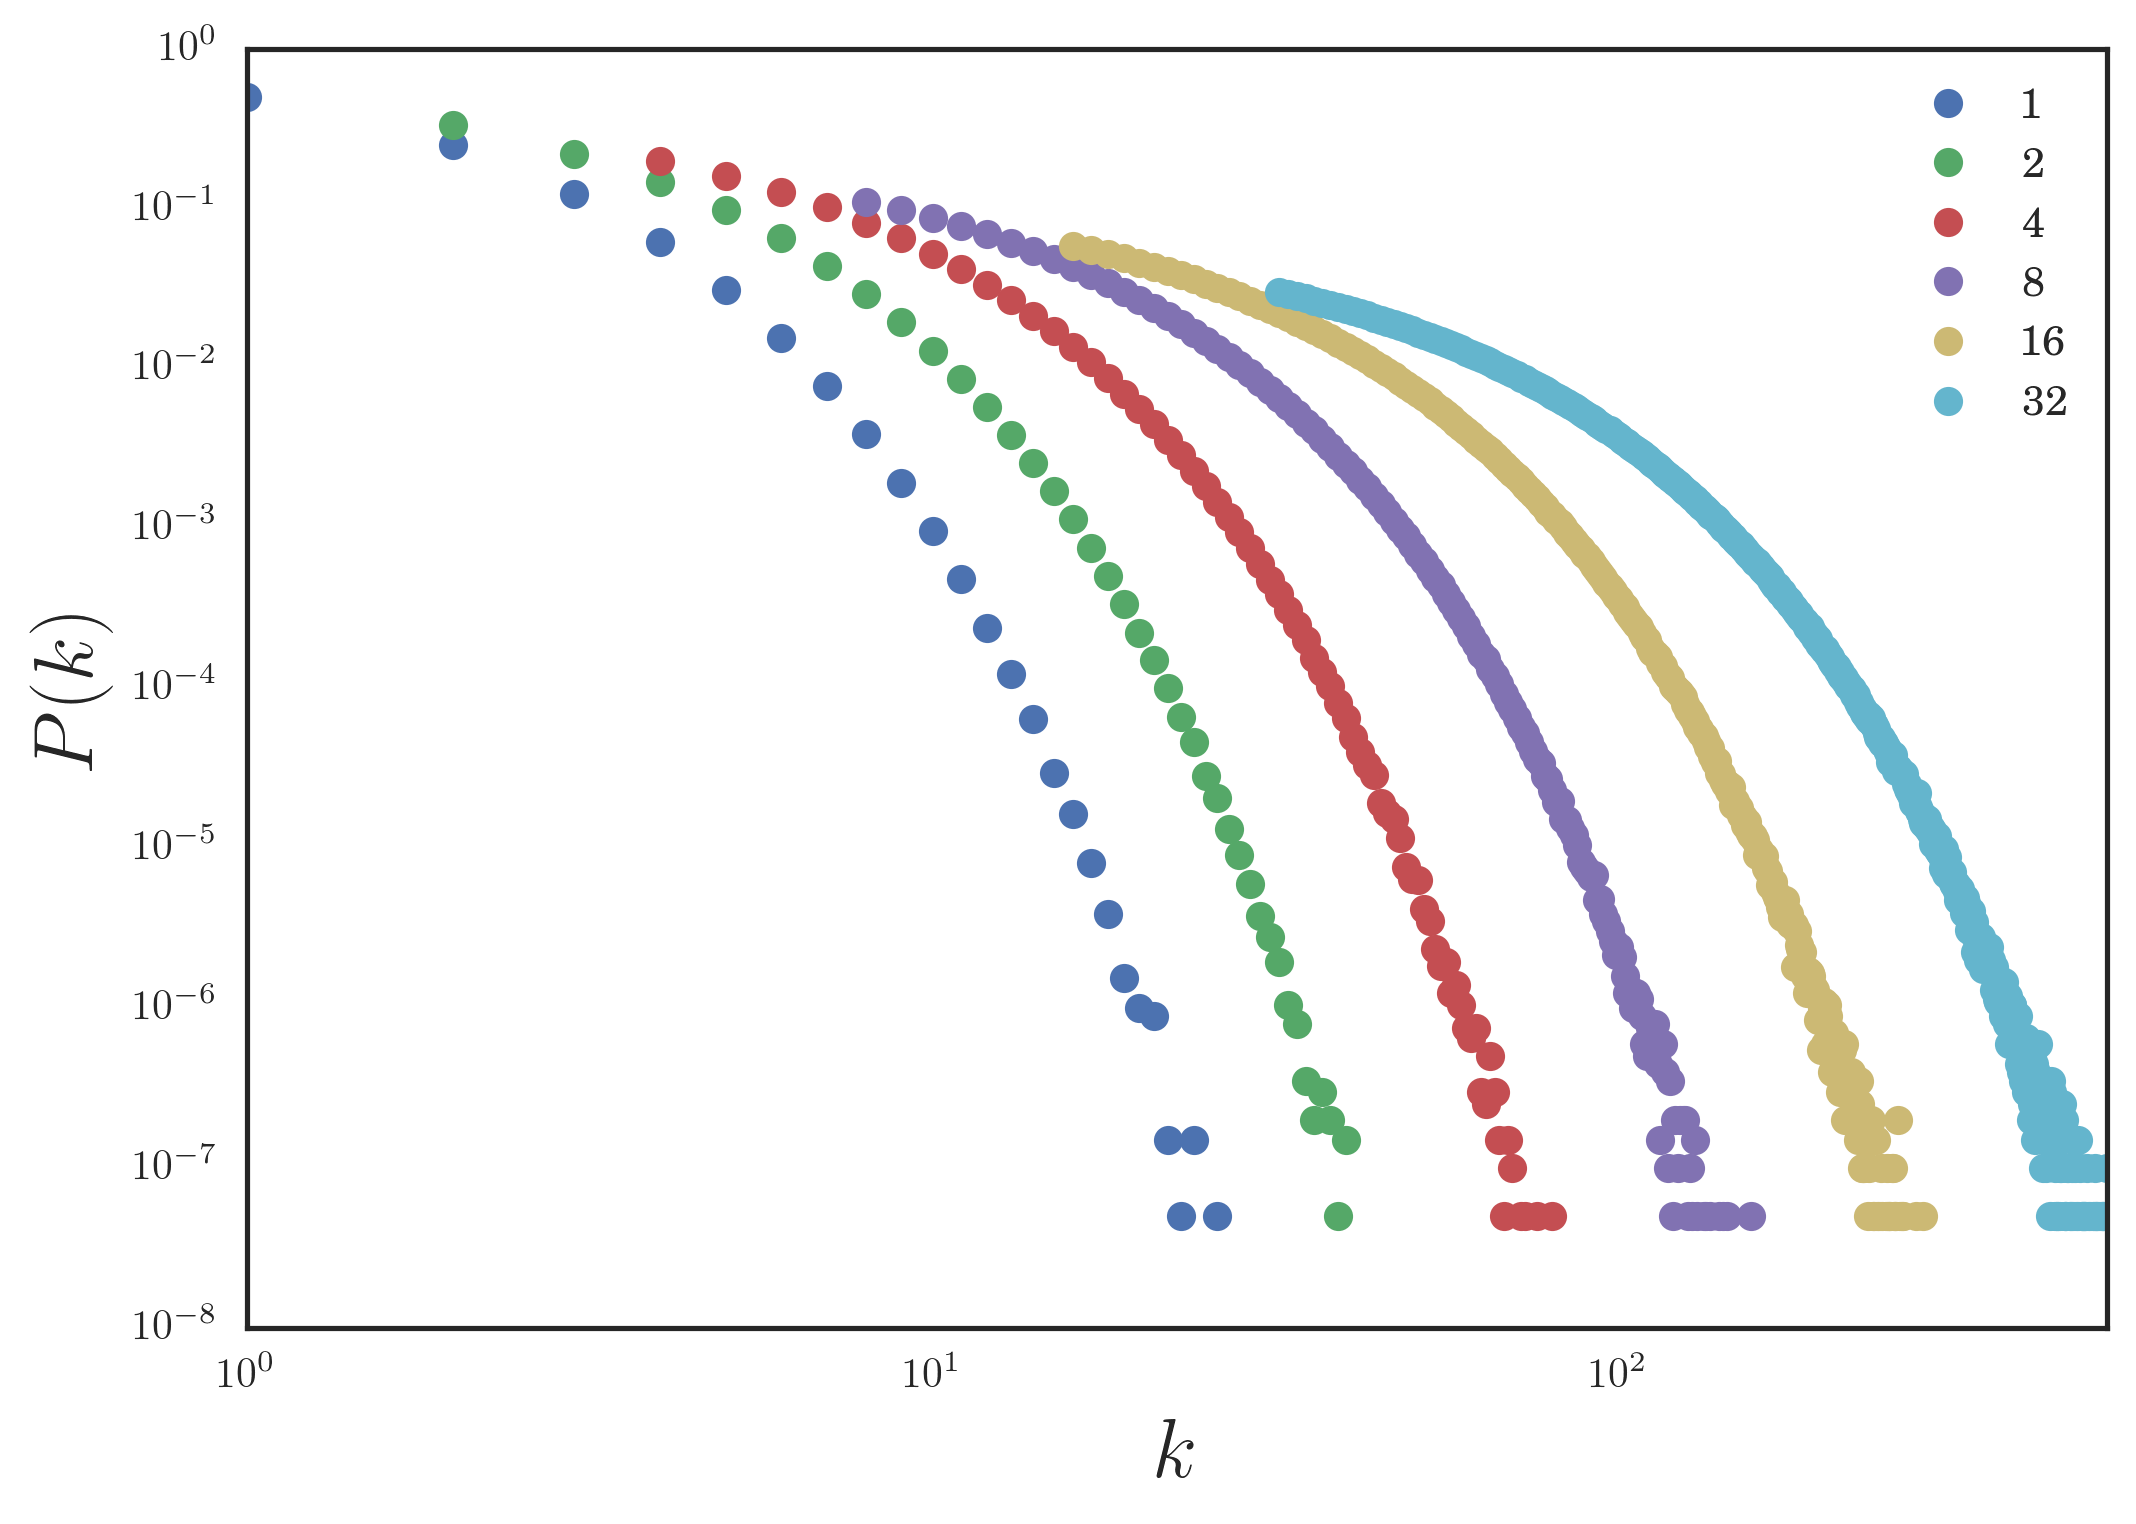
\includegraphics[height=0.5\linewidth]{img/ra-fixed-n-degree-dist}
    \caption{Raw degree distribution for random attachment for $N = 10^6$ and $m = 1, 2, 4, 8, 16, 32$. }
    \label{fig:ra-fixed-n-degree-dist}
\end{figure}

\begin{figure}
    \centering
    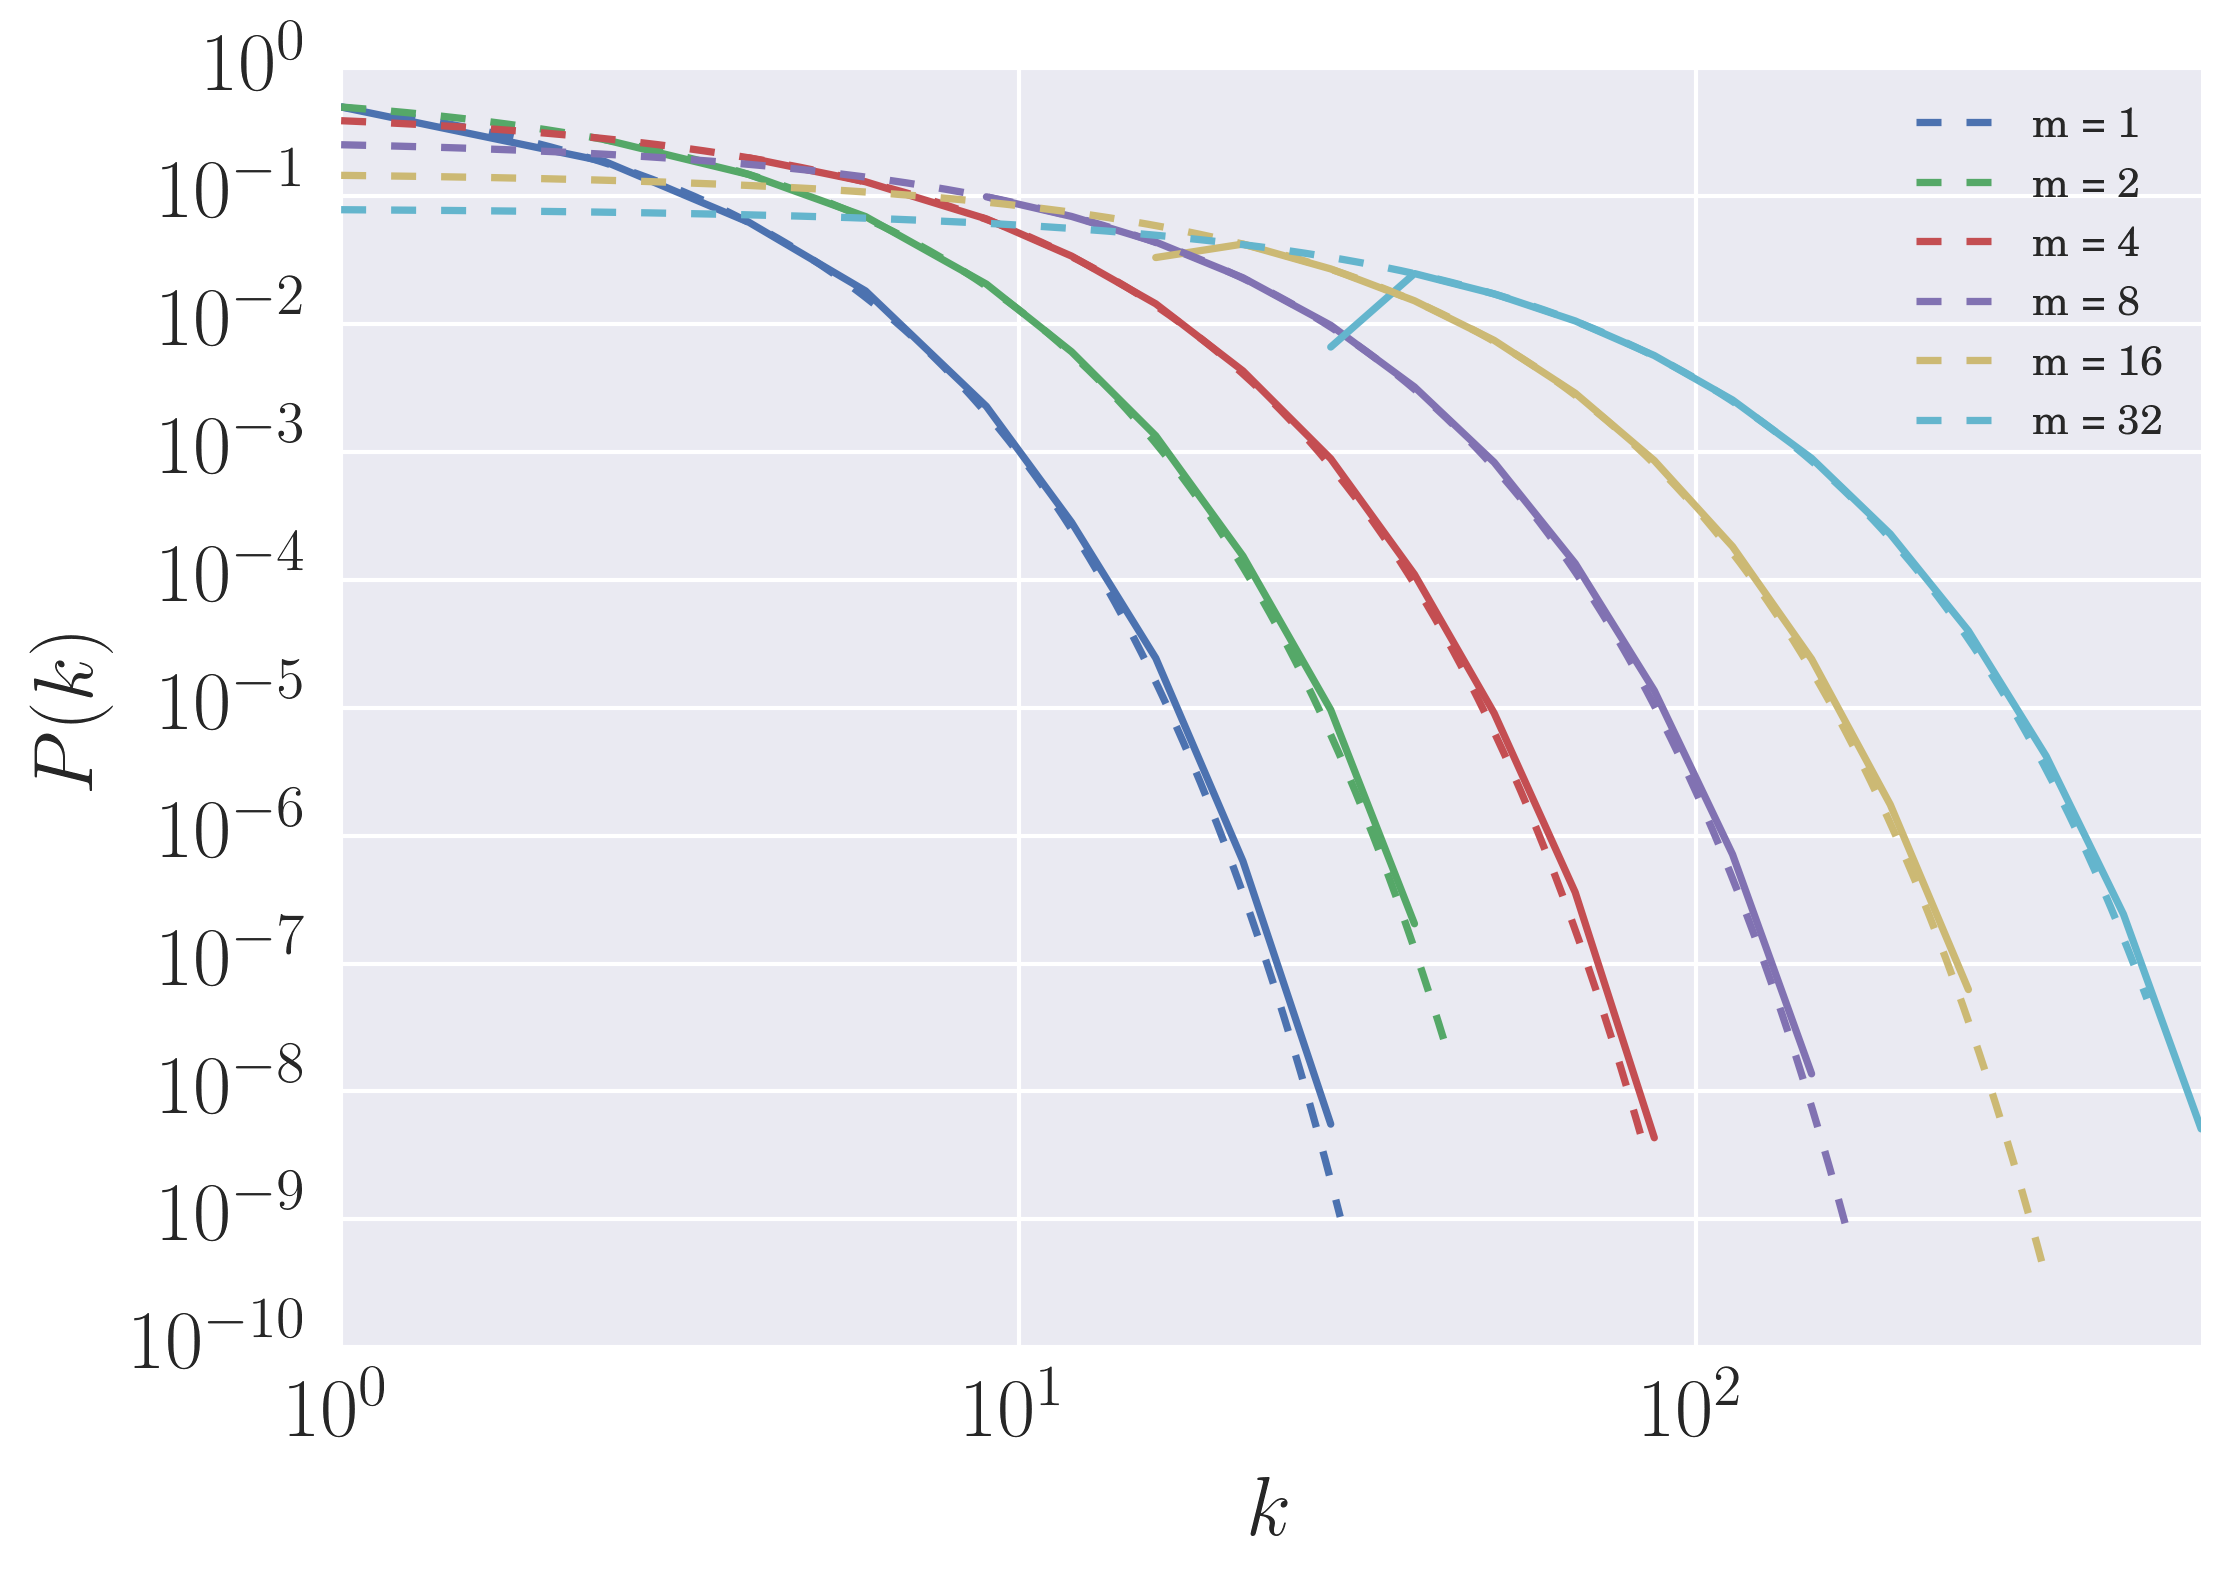
\includegraphics[height=0.5\linewidth]{img/ra-fixed-n-logbin}
    \caption{Data collapse of the degree distribution for networks of size $N=10^2, 10^3, 10^4, 10^5, 10^6, 10^7$}
    \label{fig:ra-fixed-n-logbin}
\end{figure}

Goodness of fit was tested in the same way as in the previous section. When tested against the null hypothesis of a geometric distribution governed by \autoref{eq:p-infinity-solution-ra} p-values obtained are listed below, showing that it is plausible that the simulated data follow the theoretical distribution. While the $p$-values fluctuate between 0.4 and 0.7, they are all safely above the threshold of $0.1$. 

\begin{center}
\begin{tabular}{ c | c }
N & $k_1^{\text{theory}}$ & $k_1^{\text{numerical}}$ & $k_1^{\text{numerical}} / k_1^{\text{theory}} $\\ 
\hline
1  & 0.714
2  & 0.446
4  & 0.502
8  & 0.706
16 & 0.456
\end{tabular}
\label{table:ra-ks-test}
\captionof{table}{The list of $p$-values for each $m$ for random attachment when compared with synthetic datasets.}}
\end{center}

To demonstrate whether this test is effective, random attachment simulation data was also tested against the power law distribution, and we obtained result of $p = 0$, to an accuracy of $\pm 0.05$, for all $m$. This shows that we can reject the power law hypothesis as expected. 

\subsection{Largest expected degree}\label{subsection:largest-expected-degree}
\subsubsection{Theory}
Using the same definition from the previous section for largest expected degree, we need

\begin{equation}
	N \sum_{k=k_1}^\infty p_{\infty}(k) = N \sum_{k=k_1}^\infty \frac{1}{m+1} \left (\frac{m}{m+1} \right )^{k-m} = 1.
	\label{eq:largest-expected-degree-ra-criteria}
\end{equation}

Again, the summation is similar to the previous \autoref{eq:ra-geom-series} just with a different lower limit. Applying the geometric series summation formula to the terms in the summation, we get 
\begin{equation}
	\frac{N}{m+1} \left ( \frac{m}{m+1} \right )^{k_1 - m} \frac{1}{1 - (m / (m+1))} = 1
\end{equation}

Rearranging this and taking logarithm of both sides, we obtain an expression for $k_1$:
\begin{equation}
	k_1 = \frac{\ln N}{\ln (m+1) - \ln m} + m
	\label{eq:largest-degree-ra}
\end{equation}
From this, we know that the largest degree grow logarithmically with $N$, as opposed to a power law like for preferential attachment. 

\subsubsection{Numerical analysis}
The numerical largest degree was calculated in the same way as described in the previous section. Figure ?? shows the discrepancy between the numerical and theoretical largest degree. The ratio between $k_1^{\text{theory}}$ and $k_1^{\text{numerical}}$ is largely constant. From \autoref{fig:ra-numerical-theoretical-k1} we can see that the difference between the numerical and theoretical values decrease as $N$ increases, which is expected. 

\begin{figure}
    \centering
    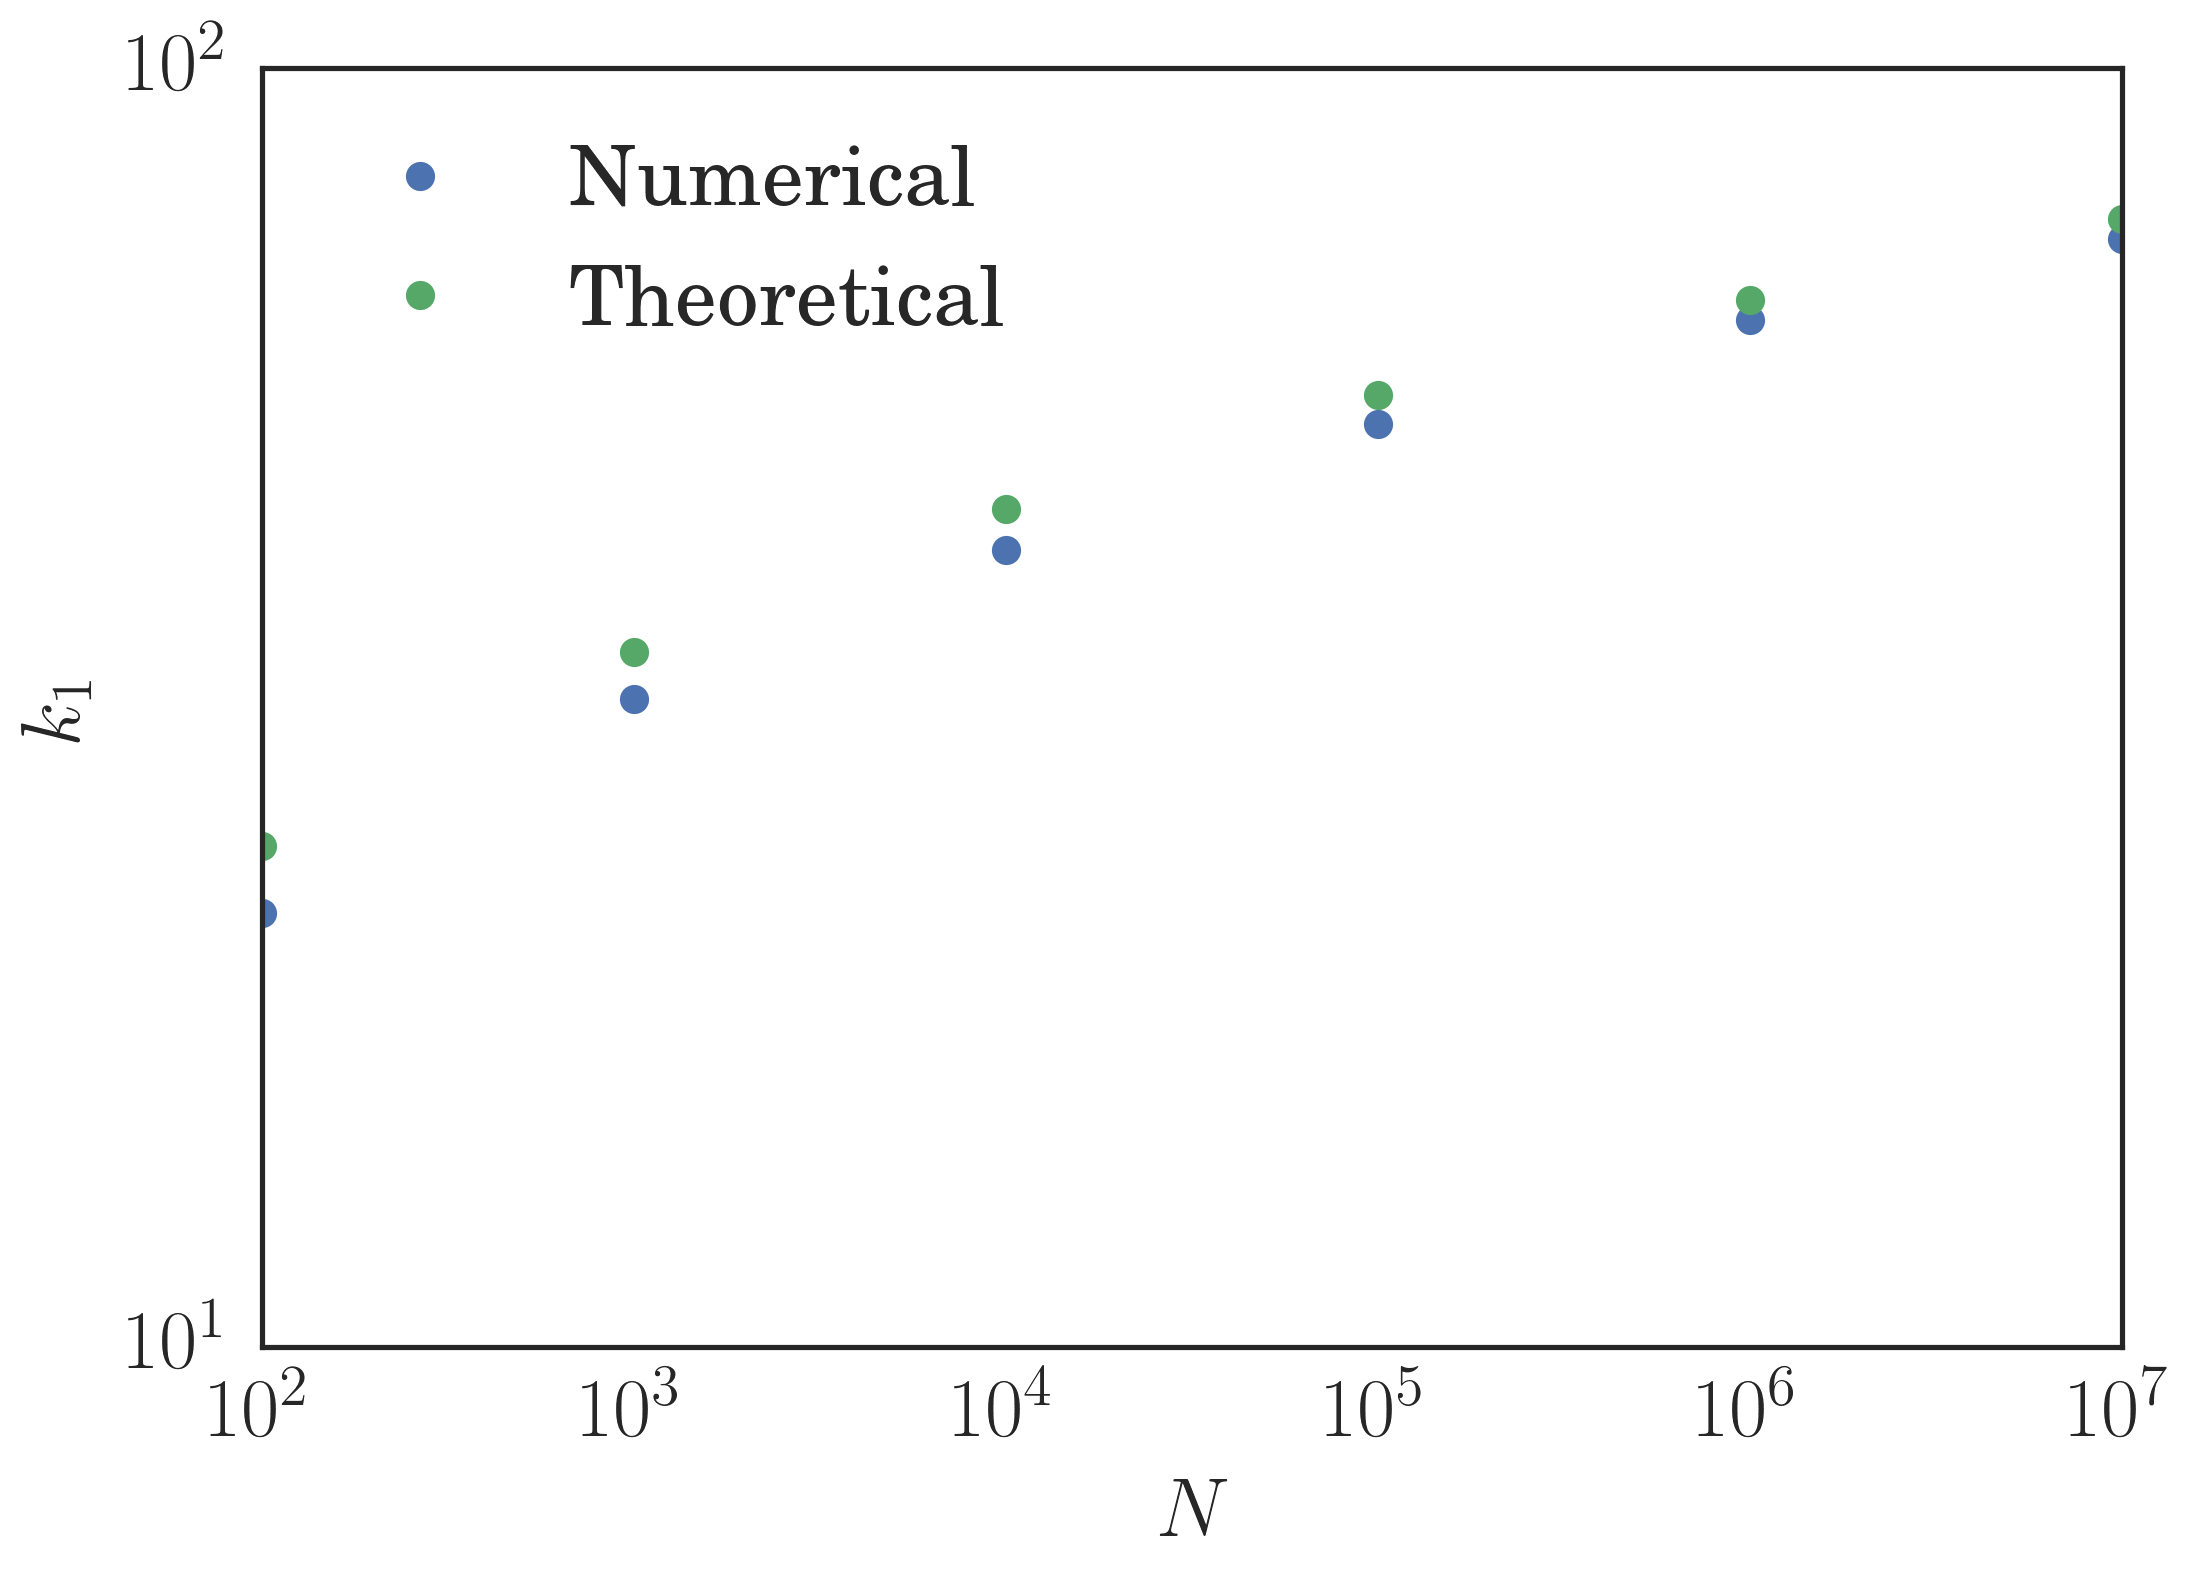
\includegraphics[height=0.5\linewidth]{img/ra-numerical-theoretical-k1}
    \caption{This shows the difference in $k_1$ for different values of $N$ ranging from $100$ to $10^7$ for random attachment. From the graph we can see that the difference between the theoretical and numerical values decrease as $N$ increases.}
    \label{fig:ra-numerical-theoretical-k1}
\end{figure}

From the following tables of values, we can also see that the values get closer to 1 for larger $N$. Similarly, the standard error was estimated from the sample standard deviation, governed by \autoref{eq:population-std}. 

\begin{center}
\begin{tabular}{ ||c | c | c | c ||}
\hline
N & $k_1^{\text{theory}}$ & $k_1^{\text{numerical}}$ & $k_1^{\text{numerical}} / k_1^{\text{theory}} $\\ 
\hline
$10^2$ & 25    & 21.85  $\pm$ 0.01 & 0.887 \\  
$10^3$ & 35   & 32.15 $\pm$ 0.03 & 0.920 \\
$10^4$ & 46   & 42.05   $\pm$  0.03  & 0.929 \\
$10^5$ & 56  & 52.75  $\pm$  0.02  & 0.949 \\
$10^6$ & 66  & 63.55  $\pm$  0.02  & 0.964 \\
$10^7$ & 76 & 73.55 $\pm$ 0.03  & 0.965 \\  
\hline
\end{tabular}
\label{table:ra-numerical-theoretical-ratio}
\captionof{table}{This table shows the theoretical and numerical values for the largest expected degree as defined in \autoref{eq:largest-degree-ra} for random attachment. The errors on $k_1$ are rounded off to 1 significant figure. }
\end{center}